\documentclass[a4paper]{article}
\usepackage[affil-it]{authblk}
\usepackage{amsthm,amsmath,amssymb}
\usepackage{geometry}
\usepackage{hyperref}
\usepackage{tikz}
\geometry{margin=1.5cm, vmargin={0pt,1cm}}
\setlength{\topmargin}{-1cm}
\setlength{\paperheight}{29.7cm}
\setlength{\textheight}{25.3cm}
\usepackage{pgfplots}
\renewcommand{\qed}{\hfill \boxed{\mathbb{Q.E.D.}}}

\tikzset{elegant/.style={smooth,thick,solid,black}}
\tikzset{eaxis/.style={smooth,thick,solid,black}}
\begin{document}
% =================================================
\title{Numerical Analysis Homework 4}

\author{Chen Wanqi 3220102895
  \thanks{Electronic address: \texttt{3220102895@zju.edu.cn}}}
\affil{Information and Computer Science 2201, Zhejiang University }


\date{\today}

\maketitle

% =============================================== 
\section*{Problem I.}

\textbf{Solution.}
\((477)_{10} = (111011101)_2 = (1.11011101)_2 \times 2^8\)


% ==========================
\section*{Problem II.}

\textbf{Solution.}
\(\frac{3}{5} = (0.100\dot{1}\dot{1}\dot{0}\dot{0})_2 = (1.00\dot{1}\dot{1}\dot{0}\dot{0})_2 \times 2^{-1} \)


The dots above the number indicate the cycle of the number.

% ==========================
\section*{Problem III.}

\begin{proof}
    Let \(x = (1.00\ldots00)_{\beta} \times \beta^e\), representing \(x\) as a normalized floating-point number.
    
    Thus, the left adjacent floating-point number is given by 
    \[
    x_L = ((\beta-1).(\beta-1)\ldots(\beta-1))_{\beta} \times \beta^{e-1}.
    \]
    
    Similarly, the right adjacent floating-point number is 
    \[
    x_R = (1.00\ldots01)_{\beta} \times \beta^e.
    \]
    
    Now consider the equation to prove:
    \[
    LHS = x_R - x = (0.00\ldots01)_{\beta} \times \beta^e .
    \]
    
    \[
    RHS = \beta \cdot (x - x_L) = \beta \cdot (0.00\ldots01)_{\beta} \times \beta^{e-1} = (0.00\ldots01)_{\beta} \times \beta^e.
    \]

    Thus, LHS = RHS, proving the equation.
\end{proof}

% ==========================
\section*{Problem IV.}

\textbf{Solution.}

From Problem II, we know that:
\[
\frac{3}{5} = (1.00\dot{1}\dot{1}\dot{1}\dot{0}\dot{0})_2 \times 2^{-1}.
\]

Under the IEEE 754 single-precision format, the left and right adjacent normalized floating-point numbers are:
\[
x_{L} = (1.0011001100110011001100)_2 \times 2^{-1},
\]
\[
x_{R} = (1.0011001100110011001101)_2 \times 2^{-1}.
\]

Now, consider the differences between these values:
\[
x - x_{L} = (1.100\dot{1}\dot{1}\dot{0}\dot{0})_2 \times 2^{-23} = \frac{8}{5} \times 2^{-23}.
\]

For \(x_{R} - x\), we compute:
\[
x_{R} - x = (x_{R} - x_{L}) - (x - x_{L})  = 2^{-22} - \frac{8}{5} \times 2^{-23} = \frac{2}{5} \times 2^{-23}.
\]

Clearly, we observe:
\[
x_{R} - x < x - x_{L}.
\]

Thus, according to the IEEE 754 rounding rule, \(\text{fl}(x) = x_{R}\).

Finally, the relative error is calculated as:
\[
\frac{x_{R} - x}{x} = \frac{2}{3} \times 2^{-23}.
\]


% ==========================
\section*{Problem V.}

\textbf{Solution.}

The unit roundoff, \(\epsilon_m\), is defined as the smallest difference between two consecutive normalized floating-point numbers. It can be calculated using the formula:  
\[
\epsilon_m = \beta^{1-t},
\]
where \(\beta\) is the base (for binary floating-point numbers, \(\beta = 2\)) and \(t\) is the number of significant digits in the mantissa.

For the IEEE 754 single-precision format, the mantissa has \(t = 24\) bits (including the implicit leading 1). Thus, the unit roundoff is:  
\[
\epsilon_m = 2^{1-24} = 2^{-23}.
\]


% ==========================

\section*{Problem VI.}

\textbf{Solution.}

Let \(u = 1\) and \(v = \cos(x)\), where \(x = \frac{1}{4}\). We compute:
\[
1 - \frac{v}{u} = 1 - \cos\left(\frac{1}{4}\right) \approx 0.031088.
\]

This value satisfies the inequality:
\[
2^{-6} \leq 0.031088 \leq 2^{-5}.
\]

According to Theorem 4.49, the number of most significant digits lost in the subtraction \(u - v = 1 - \cos(x)\) is at most 6 and at least 5.


% ==========================

\section*{Problem VII.}

\textbf{Solution.}

Two alternative methods can be used:

\textbf{Method 1: Trigonometric Identity:}  
Using the identity \(1 - \cos(x) = 2\sin^2\left(\frac{x}{2}\right)\) .

\textbf{Method 2: Taylor Series Expansion:}  
For small values of \(x\), the Taylor series expansion of \(\cos(x)\) can be used:
\[
1 - \cos(x) \approx \frac{x^2}{2} - \frac{x^4}{24}.
\]

% ==========================
\section*{Problem VIII.}

\textbf{Solution.}

\textbf{(1) \(f(x) = (x - 1)^{\alpha}\):}

\[
C_f(x) = \left|\frac{xf'(x)}{f(x)}\right| = \left|\frac{\alpha x}{x - 1}\right|.
\]

When \(\alpha \neq 0\), \(C_f(x) \to \infty\) as \(x \to 1^+\) or \(x \to 1^-\).  

When \(\alpha = 0\), \(C_f(x) = 0\), which remains finite.

\textbf{(2) \(f(x) = \ln(x)\):}

\[
C_f(x) = \left|\frac{xf'(x)}{f(x)}\right| = \left|\frac{1}{\ln(x)}\right|.
\]

\(C_f(x) \to \infty\) as \(x \to 0^+\).  

\textbf{(3) \(f(x) = e^x\):}

\[
C_f(x) = \left|\frac{xf'(x)}{f(x)}\right| = |x|.
\]

\(C_f(x) \to \infty\) as \(x \to \pm \infty\).

\textbf{(4) \(f(x) = \arccos(x)\):}

\[
C_f(x) = \left|\frac{xf'(x)}{f(x)}\right| = \left|\frac{x}{\arccos(x) \sqrt{1 - x^2}}\right|.
\]

\(C_f(x) \to \infty\) as \(x \to \pm 1\).


% ==========================
\section*{Problem IX.}

\textbf{Solution.}

\textbf{(1):}  

\(f(x) = 1 - e^{-x}\)  

\[
cond_f(x) = \left|\frac{xf'(x)}{f(x)}\right| = \left|\frac{xe^{-x}}{1 - e^{-x}}\right|.
\]

For \(x \in [0,1]\),  
\[
cond_f(x) = \frac{xe^{-x}}{1 - e^{-x}}.
\]

To find the maximum of \(cond_f(x)\), let  
\[
cond_f'(x) = \frac{e^{-x}[(1-x)(1-e^{-x}) - xe^{-x}]}{(1 - e^{-x})^2} > 0.
\]

Simplifying the numerator:  
\[
(1-x)(1-e^{-x}) - xe^{-x} > 0,
\]
which reduces to  
\[
x + e^{-x} < 1.
\]

The left-hand side (\(x + e^{-x}\)) is an increasing function for \(x \in [0,1]\).  

Thus, the maximum value of \(cond_f(x)\) is attained at \(x = 1\):  
\[
\lim_{x \to 1} cond_f(x) = 1.
\]

Therefore, \(cond_f(x) \leq 1\) for \(x \in [0,1]\).

\textbf{(2):}

Let \( f(x) = 1 - e^{-x} \), and the computed result be:  
\[
f_A(x) = (1 - e^{-x}(1 + \delta_1))(1 + \delta_2),
\]
where \( |\delta_1|, |\delta_2| \leq \epsilon_u \).

Expanding:
\[
f_A(x) = (1 - e^{-x}) + \delta_2(1 - e^{-x}) - \delta_1 e^{-x}(1 + \delta_2).
\]

The relative error is:
\[
\delta(x) = \delta_2 - \frac{\delta_1(1 + \delta_2)}{e^x - 1}.
\]

Taking absolute values:
\[
|\delta(x)| \leq \epsilon_u + \frac{\epsilon_u (1 + \epsilon_u)}{e^x - 1}.
\]

Simplifying:
\[
|\delta(x)| \leq \epsilon_u \phi(x), \quad \phi(x) = \frac{e^x}{e^x - 1}.
\]

From Theorem 4.78:
\[
\text{cond}_A(x) \leq \frac{\phi(x)}{C_f(x)} = \frac{e^x}{x}.
\]


\textbf{(3):}

We plot the graph of the function \(\frac{e^x}{x}\) and \(cond_f(x)\) in the range \([0,1]\) with python to compare their values.

\begin{tikzpicture}
  \begin{axis}[
      width=12cm, height=8cm,
      xlabel={$x$},
      ylabel={Condition Number},
      xmin=0, xmax=1,
      ymin=0, ymax=60,
      legend pos=north west,
      grid=major,
      grid style={dashed,gray!30},
      tick label style={font=\small},
      legend style={font=\small},
  ]

  % Plot cond_f(x)
  \addplot[
      domain=0.01:1, 
      samples=200, 
      thick, 
      blue
  ]
  {x * exp(-x) / (1 - exp(-x))};
  \addlegendentry{$\text{cond}_f(x)$};

  % Plot Upper Bound of cond_A(x)
  \addplot[
      domain=0.01:1, 
      samples=200, 
      thick, 
      red, 
      dashed
  ]
  {exp(x) / x};
  \addlegendentry{Estimated Upper Bound of $\text{cond}_A(x)$};

  \end{axis}
\end{tikzpicture}


% ==========================

\section*{Problem X.}

\begin{proof}

  We start from the definition of the matrix 2-norm:  
  \[
  \|A\|_2 = \sup_{\|x\|_2 \neq 0} \frac{\|Ax\|_2}{\|x\|_2},
  \]
  which means that the 2-norm of a matrix is the maximum factor by which it stretches the 2-norm of a vector. Using the Singular Value Decomposition (SVD), any matrix \(A\) can be written as \(A = U \Sigma V^*\), where \(U\) and \(V\) are unitary matrices, and \(\Sigma = \text{diag}(\sigma_1, \sigma_2, \dots, \sigma_n)\) is a diagonal matrix of singular values, ordered such that \(\sigma_1 \geq \sigma_2 \geq \cdots \geq \sigma_n \geq 0\).
  
  For any nonzero vector \(x\), we have:
  \[
  \|Ax\|_2 = \|U \Sigma V^* x\|_2 = \|\Sigma V^* x\|_2,
  \]
  because the unitary matrix \(U\) preserves the 2-norm. Let \(y = V^*x\), so that \(\|y\|_2 = \|x\|_2\) (since \(V\) is also unitary), and we get:
  \[
  \|\Sigma y\|_2 = \sqrt{\sum_{i=1}^n \sigma_i^2 y_i^2} \leq \sigma_1 \|y\|_2 = \sigma_1 \|x\|_2.
  \]
  Equality is achieved when \(y = [1, 0, \dots, 0]^\top\). Thus, the 2-norm of the matrix is given by its largest singular value:
  \[
  \|A\|_2 = \sigma_1 = \sigma_{\text{max}}.
  \]
  
  Similarly, for the inverse of \(A\), the 2-norm is determined by the reciprocal of the smallest singular value:
  \[
  \|A^{-1}\|_2 = \frac{1}{\sigma_{\text{min}}},
  \]
  where \(\sigma_{\text{min}}\) is the smallest nonzero singular value (since \(A\) is nonsingular).
  
  The condition number of \(A\) is therefore:
  \[
  \text{cond}_2(A) = \|A\|_2 \|A^{-1}\|_2 = \frac{\sigma_{\text{max}}}{\sigma_{\text{min}}}.
  \]
  
  If \(A\) is normal (i.e., \(A A^* = A^* A\)), then the singular values of \(A\) are equal to the moduli of its eigenvalues. Hence, we can write:
  \[
  \sigma_{\text{max}} = |\lambda_{\text{max}}|, \quad \sigma_{\text{min}} = |\lambda_{\text{min}}|,
  \]
  where \(\lambda_{\text{max}}\) and \(\lambda_{\text{min}}\) are the eigenvalues of \(A\) with the largest and smallest moduli, respectively. In this case, the condition number becomes:
  \[
  \text{cond}_2(A) = \frac{|\lambda_{\text{max}}|}{|\lambda_{\text{min}}|}.
  \]
  
  Finally, if \(A\) is unitary, all of its eigenvalues have modulus 1, and thus:
  \[
  \text{cond}_2(A) = \frac{|\lambda_{\text{max}}|}{|\lambda_{\text{min}}|} = 1.
  \]
  
  This completes the proof.

\end{proof}


% ==========================
\section*{Problem XI.}

\textbf{Solution.}

As \(r\) is the root of the polynomial \(q(r) = r^n + a_{n-1}r^{n-1} + \cdots + a_0\), we have:

\[
r^n + a_{n-1}r^{n-1} + \cdots + a_0 = 0.
\]

Differentiating \( q(r) \) with respect to \( a_i \), we obtain 

\[
\frac{\partial}{\partial a_i} \big(r^n + a_{n-1}r^{n-1} + \cdots + a_0\big) = 0,
\]

which leads to 

\[
\frac{\partial r}{\partial a_i} \big(nr^{n-1} + a_{n-1}(n-1)r^{n-2} + \cdots + 2a_2r + a_1\big) + r^i = 0.
\]

Rearranging gives 

\[
\frac{\partial r}{\partial a_i} = \frac{-r^i}{nr^{n-1} + a_{n-1}(n-1)r^{n-2} + \cdots + 2a_2r + a_1} = \frac{-r^i}{q'(r)},
\]

where \( q'(r) \) is the derivative of \( q(r) \) with respect to \( r \). The componentwise condition number is defined as 

\[
\text{cond}_f(x) = \frac{1}{|r|} \bigg| \sum_{i=0}^{n-1} a_i \frac{\partial r}{\partial a_i} \bigg|.
\]

Substituting \( \frac{\partial r}{\partial a_i} = \frac{-r^i}{q'(r)} \), we have 

\[
\text{cond}_f(x) = \frac{1}{|r|} \bigg| \sum_{i=0}^{n-1} \frac{-a_i r^i}{q'(r)} \bigg|.
\]

Using \( q(r) = 0 \), we know 

\[
\sum_{i=0}^{n-1} a_i r^i = -r^n.
\]

Substituting this result simplifies the condition number to 

\[
\text{cond}_f(x) = \frac{1}{|r|} \bigg| \frac{-r^n}{q'(r)} \bigg| = \bigg| \frac{r^{n-1}}{q'(r)} \bigg|.
\]

Thus, the componentwise condition number of \( f \) is 

\[
\text{cond}_f(x) = \bigg| \frac{r^{n-1}}{q'(r)} \bigg|.
\]

In Wilkinson example,assume that r is the foot of f(x)

$$f(x)=\prod_{k=1}^p(x-k)$$
$$cond_f(r)=\frac{r^p}{f'(r)}$$

Hence,it has the same result with Wilkinson,a small change of the coefficient
of the polynomial would cause a large change of the root.

% ==========================
\section*{Problem XII.}

\textbf{Solution.}

Assume \(\beta = 2\), \(p = 2\), \(L = -1\), and \(U = 1\), with \(a = (1.0)_2 = 1\) and \(b = (1.1)_2 = 1.5\). 

The exact division \(\frac{a}{b} = \frac{1}{1.5} = \frac{2}{3}\) in binary is \(0.101010\ldots_2\). 

Rounding this to two bits of precision results in \( \text{fl}\left( \frac{a}{b} \right) = 0.10_2 = 0.5 \). 

The relative error is then \( E_{rel} = \left| \frac{0.5 - \frac{2}{3}}{\frac{2}{3}\ldots} \right| = \frac{1}{4} \), which equals the unit roundoff \(\epsilon_u = 2^{-2} = 0.25\). 

This contradicts Lemma 4.39, which states that the error should be strictly less than \( \epsilon_u \).


% ==========================
\section*{Problem XIII.}

\textbf{Solution.}

We start with the interval [128, 129]. In IEEE 754 single-precision floating point representation:

\[
128 = (1.000\ldots)_2 \times 2^7
\]
\[
129 = (1.00000010\ldots)_2 \times 2^7
\]

The absolute error \(E_{abs}\) is:

\[
E_{abs} = (0.00\ldots1)_2 \times 2^7 = 2^{-23} \times 2^7 = 2^{-16}
\]

Approximating this, we get:

\[
E_{abs} \approx 1.526 \times 10^{-5}
\]

Since \(E_{abs} > 10^{-6}\), it is not possible to compute the root with an accuracy of \(10^{-6}\).



% ==========================

\section*{Problem XIV.}

\textbf{Solution.}

In the case of cubic splines, the matrix involved is typically a tridiagonal matrix that arises from solving a system of equations to determine the spline coefficients. When the distance between two adjacent points is much smaller than the others, the corresponding entries in the matrix become very small, which leads to a matrix with a high condition number. As a result, the solution becomes more sensitive to small perturbations in the data, causing large inaccuracies in the curve fitting.


% ==========================
\section*{Excercise 4.33.}

\textbf{Solution.}

\textbf{Case 1 :}

For $a = 1.234 \times 10^4$ and $b = 8.769 \times 10^4$

(i) $b \leftarrow 8.769 \times 10^4, e_c \leftarrow 4.$

(ii) $m_c \leftarrow 10.003.$

(iii) $m_c \leftarrow m_c / \beta = 1.0003, e_c \leftarrow e_c + 1 = 5$.

(iv) Do nothing.

(v) $m_c \leftarrow 1.000$

(vi) $c \leftarrow 1.000 \times 10^5$

Result: $c = 1.000 \times 10^5$

\textbf{Case 2 :}

For $a = 1.234 \times 10^4$ and $b = -5.678 \times 10^0$

(i) $b \leftarrow -0.0005678 \times 10^4, e_c \leftarrow 4.$

(ii) $m_c \leftarrow 1.2334322.$

(iii) Do nothing.

(iv) Do nothing.

(v) $m_c \leftarrow 1.233$

(vi) $c \leftarrow 1.233 \times 10^4$

Result: $c = 1.233 \times 10^4$

\textbf{Case 3 :}

For $a = 1.234 \times 10^4$ and $b = -5.678 \times 10^-3$

Result: $c = 1.234 \times 10^4$


% ==========================
\section*{Excercise 4.42.}

The rounding error \(\delta\) in the floating-point result of the sum is given by:

\[
\text{fl}\left( \sum_{i=0}^{n} a_i \right) = \left( 1 + \delta \right) \sum_{i=0}^{n} a_i
\]

In floating-point arithmetic, each addition introduces a small error due to the limited precision of number representation. When adding smaller numbers first, the rounding error does not significantly affect the larger numbers, as their magnitude dominates the operation. 

By summing the smaller numbers first, the errors accumulate in a way that their impact on the final sum is minimized. On the other hand, if larger numbers are added first, the rounding error in the smaller numbers is amplified, as the larger numbers introduce relatively more significant rounding errors that can affect the smaller terms.

Thus, by sorting the numbers \(a_i\) in increasing order and summing them in that order, we ensure that the rounding errors in the smaller numbers do not propagate and compound in a way that would cause a larger total error.



% ==========================
\section*{Excercise 4.43.}
First, consider each term \( a_ib_i \) being calculated in floating-point arithmetic. The result of the multiplication is subject to a rounding error:
\[
\text{fl}(a_i b_i) = (a_i b_i)(1 + \delta_i^{(1)}),
\]
where \( |\delta_i^{(1)}| \leq \epsilon \), the machine epsilon.

The floating-point addition of two terms, such as \( \text{fl}(a_1b_1) + \text{fl}(a_2b_2) \), introduces another rounding error:
\[
\text{fl}(a_1b_1 + a_2b_2) = \left(\text{fl}(a_1b_1) + \text{fl}(a_2b_2)\right)(1 + \delta_1^{(2)}),
\]
where \( |\delta^{(2)}| \leq \epsilon \). Extending this to the full expression \( \text{fl}(a_1b_1 + a_2b_2 + a_3b_3) \), we have:
\[
\text{fl}(a_1b_1 + a_2b_2 + a_3b_3) = [[(a_1b_1)(1 + \delta_1^{(1)}) + (a_2b_2)(1 + \delta_2^{(1)})](1 + \delta_1^{(2)}) + (a_3b_3)(1 + \delta_3^{(1)})](1 + \delta_2^{(2)}).
\]

The corresponding derivation for \( \text{fl}\left(\sum_i \prod_j a_{i,j}\right) \) follows similar logic. Each product \( \prod_j a_{i,j} \) introduces a sequence of multiplicative rounding errors:
\[
\text{fl}\left(\prod_j a_{i,j}\right) = \left(\prod_j a_{i,j}\right) \prod_k (1 + \delta_{i,k}^{(1)}).
\]
Adding these products introduces further rounding errors:
 
\[
  \text{fl}\left(\sum_i \prod_j a_{i,j}\right) = \left( \left( \text{fl}\left(\prod_j a_{1,j}\right) + \text{fl}\left(\prod_j a_{2,j}\right) \right)(1 + \delta_1^{(2)}) + \text{fl}\left(\prod_j a_{3,j}\right) \right)(1 + \delta_2^{(2)}) \dots
\]
  

% ==========================

\section*{Excercise 4.80.}

In this case, we are given the function

\[
f(x) = \frac{\sin x}{1 + \cos x}, \quad x \in (0, \frac{\pi}{2}).
\]

We begin by analyzing the condition number of this function. First, we compute the condition number \( \text{cond}_f(x) \) by using the definition 4.59, which gives

\[
\text{cond}_f(x) = \frac{x}{\sin x}.
\]

Next, applying Theorem 4.40 and assuming that the computations of \( \sin x \) and \( \cos x \) have relative errors within machine roundoff, we express the computed value \( f_A(x) \) as

\[
f_A(x) = \frac{\text{fl}(\sin x (1 + \delta_1))}{(1 + \delta_2) (1 + \delta_3) \text{fl}(1 + \cos x)(1 + \delta_4)}.
\]

We can simplify this expression to

\[
f_A(x) = \frac{\sin x}{1 + \cos x} \left\{ 1 + \delta_2 + \delta_4 - \delta_3 - \delta_1 \frac{1 + \cos x}{\sin x} \right\}.
\]

From this, we conclude that

\[
\varphi(x) = 3 + \frac{1 + \cos x}{\sin x},
\]

which means

\[
\text{cond}_A(x) \leq \frac{\sin x}{x} \left( 3 + \frac{1 + \cos x}{\sin x} \right).
\]

As a result, \( \text{cond}_A(x) \) may become unbounded as \( x \to 0 \), but it is bounded by a constant as \( x \to \frac{\pi}{2} \).

% =======================
\section*{References}
\begin{itemize}
   \item handoutsNumPDEs
   \item ChatGPT, *AI Language Model*, OpenAI Platform, 2024.
\end{itemize}

\end{document}